\section{Frequency and Phase Estimation}%
\label{sec:freq_est}

Frequency and phase estimation, also called carrier synchronization, is the next step after detection for coherent demodulation.
In this section, we discuss the estimation algorithm by assuming the time synchronization of the preamble is perfect, i.e., 
the observation window contains the complete preamble. For the same reason as in the detection section, we first derive the estimator
by assuming the effect of the fractional delay in signal model~\eqref{eq:model} is neglected.
In simulation section, we will discuss how much the value of fractional delay degrades the estimating accuracy of estimators by
comparing with different sampling rate.
% I forget to say in last meeting, the plot was truly obtained from a random sequence but with a good autocorrelation property.
% For this time, I compared with the reason with my previous sequence and gold sequence, the result shows the same.
% For figure 2, I think at 0 dB, since the SD estimator may not be accurate enough, the generalized correlation may not tend to be perfectly uncorrelated.
% For this reason, I just keep the previous results with some other modifications for this time.

For estimating frequency offset $\delta$ and the phasor $S=Ae^{j\phi}$, the maximum likelihood (ML) estimate of the parameters in~\eqref{eq:model} is given by

\begin{equation}
\label{eq:ML_f_S}
  \hat{\delta},\hat{S}=\min_{\delta,S=Ae^{j\phi}}\sum_{n=0}^{N-1}|r_n-s_nSe^{j2\pi\delta n}|^{2}.
\end{equation}
% extension to reviewer 1, comment 3
By taking the Wirtinger derivative with respect to $S$ and setting it equal to zero, a 
closed form for the estimated phasor $\hat{S}$ is readily derived,

\begin{equation}
    \label{eq:opt_S}
    \hat{S}=\frac{\sum_{n=0}^{N-1}{r_{n}s_n^{*}e^{-j2\pi\hat{\delta} n}}}{\sum_{n=0}^{N-1}|s_{n}|^2},
  \end{equation}
and $\hat{\phi}=\arg\{S\}$. We see the estimate of phasor $\hat{S}$ relies on the estimate of frequency $\hat{\delta}$.
It is shown later the derivation of $\hat{\delta}$ also plugs in the expression of phasor estimate in~\eqref{eq:opt_S}. Thus, the estimators for frequency and phasor are
joint estimators. Moreover, by plugging~\eqref{eq:opt_S} in~\eqref{eq:generalized_corr}, the GLRT based detector finally reduces to

\begin{equation}
  \label{eq:reduced_GLRT_detector}
  \rho(p)=
  \frac{|\hat{S}^{(\text{num})}_p|}
  {||\bm{r}_{p}||\cdot||\bm{s}||} \LRT{H_1}{H_0} \gamma
\end{equation}
where $\hat{S}^{(\text{num})}$ denotes the numerator of phasor estimate in~\eqref{eq:opt_S} and $||\bm{s}||$ is Euclidean norm of the preamble. From~\eqref{eq:reduced_GLRT_detector} to~\eqref{eq:generalized_corr}, the computational complexity is greatly decreased.

% extension to reviewer 1, comment 3, reviewer 3, comment 4
The frequency estimate is obtained similarly as the zero of the
derivative of~\eqref{eq:ML_f_S},

\begin{equation}
    \label{eq:intm_neces_cond1}
    \sum_{n=0}^{N-1}{(r_{n}s_n^{*}S^{*}ne^{-j2\pi \delta n}-s_ns_n^{*}n)=0}.
    \end{equation}
Note $\sum_{n=0}^{N-1}{s_ns_n^{*}n}$ is real
valued, which results in the imaginary part of left hand side of~\eqref{eq:intm_neces_cond1} be zero;
By plugging the estimate for $S$ of~\eqref{eq:opt_S} into~\eqref{eq:intm_neces_cond1} and rearranging the order of indexes, yields

\begin{equation}
    \label{eq:intm_neces_cond2}
    \Im\bigg\{\sum_{m=0}^{N-1}{\sum_{n=0}^{N-1}{nr_{n}r_{m}^{*}s_n^{*}s_me^{j2\pi \delta(m-n)}}}\bigg\} = 0.
  \end{equation}
A change of variables lets us focus on the difference between sampling instances $m$ and $n$.
With $k=m-n$,~\eqref{eq:intm_neces_cond2} becomes

\begin{equation}
    \label{eq:intm_neces_cond3}
    \Im\bigg\{\sum_{m=0}^{N-1}{\sum_{k{=}m-(N-1)}^{m}{(m{-}k)r_{m-k}r_{m}^{*}s_{m-k}^{*}s_me^{j2\pi \delta k}}}\bigg\}=0.
  \end{equation}
Reversing the order of summation in~\eqref{eq:intm_neces_cond3}, we get

\begin{equation}
    \begin{aligned}
    \label{eq:intm_neces_cond4}
    \Im\bigg\{&\sum_{k=-(N-1)}^{0}\sum_{m=0}^{N-1+k}{(m{-}k)r_{m-k}r_{m}^{*}s_{m-k}^{*}s_me^{j2\pi \delta k}+}\\
    &\sum_{k=1}^{N-1}\sum_{m=k}^{N-1}{(m{-}k)r_{m-k}r_{m}^{*}s_{m-k}^{*}s_me^{j2\pi \delta k}}\bigg\}= 0.
    \end{aligned}
  \end{equation}
The term for $k{=}0$ in~\eqref{eq:intm_neces_cond4} can be eliminated since it is real-valued. For $k \neq 0$, the positive and negative indices $k$ are symmetric. 
After grouping terms appropriately, the necessary condition for $\hat{\delta}$ is given by

\begin{equation}
    \label{eq:delta}
    J(\hat{\delta}) = \Im\bigg\{\sum_{k=1}^{N-1}{\sum_{m=k}^{N-1}{kr_{m-k}r_m^{*}s_{m-k}^{*}s_m}e^{j2\pi\hat{\delta}k}}\bigg\}=0.
    \end{equation}
This expression is fundamentally equivalent to conditions provided by Luise and Reggiannini~\cite{Luise_Reggiannini_95} and Fitz~\cite{Fitz_94}.
However,~\eqref{eq:delta} explicitly allows for pulse shaping and oversampling.

The estimator $\hat{\delta}$ in~\eqref{eq:delta} has no closed-form
solution.
In~\cite{Luise_Reggiannini_95}, it is approximated by replacing the exponential with its
Taylor series expansion.
In~\cite{Fitz_94}, an approximate solution is obtained via Euler's
identity for large $N$.
Both solutions have computational complexity $O(N^2)$ reflecting the
double summation.

Since our paper focus on the joint detection and estimation problem, we propose a family of alternative solutions to~\eqref{eq:delta}.
A coarse solution with $O(N)$ complexity is used for operating at the sample
rate during the sequential GLRT detection;
it prioritizes low complexity at the expense of some loss of accuracy.
A fine solution is used to improve the estimation accuracy for coherent demodulation once the preamble has been detected.
The two solutions are given with details in the next sections.

\subsection{Solution I: (Coarse) Single-Difference (SD) Estimator}

The first estimator is rooted in the insight that at high SNR environment, every lag $k$ in~\eqref{eq:delta} can be used to
approximate the true frequency offset $\bar{\delta}$. Assume noise is very small, i.e.,
$r_m \approx s_mAe^{j(2\pi \bar{\delta} m+\phi)}$, and~\eqref{eq:delta} can be expanded to

\begin{equation}
    \label{eq:delta_extens_no_noise}
    \Im\bigg\{A^2\sum_{k=1}^{N-1}\sum_{m=k}^{N-1}k|s_{m-k}|^2|s_m|^2e^{j2\pi (\hat{\delta}-\bar{\delta})k}\bigg\}=0.
    \end{equation}
Note that in~\eqref{eq:delta_extens_no_noise} the inner summation is purely real for every lag~$k$ if $\hat{\delta}=\bar{\delta}$.
This observation suggests that an unbiased estimate of the frequency offset can be obtained by using only a single lag~$k$
from~\eqref{eq:delta}. The approach lowers the complexity from $O(N^2)$ to $O(N)$ and permits a closed-form solution for $\hat{\delta}$.  
The disadvantage of the estimator by using single lag $k$ is its insufficient estimating accuracy since it lacks of the processing gain by outer integrator.
Thus, the estimator is named as the coarse SD estimator. We just omit "coarse" for simplicity from now.
However, due to the low complexity, the SD estimator can be used for 
frequency offset correction of sequential GLRT detector in~\eqref{eq:generalized_corr}. 

\subsubsection{Closed-form expression} 
For one lag $k$, the primary SD estimator is directly obtained by reducing~\eqref{eq:delta_extens_no_noise},
\begin{equation}
    \label{eq:delta_SD}
    \est{\delta}{\text{primary}-\sd}(k)=-\frac{\arg\big\{\sum_{m=k}^{N-1}r_{m-k}r_m^*s_{m-k}^*s_m\big\}}{2\pi k}.
\end{equation}

\subsubsection{Performance of primary SD estimator}
In low (or moderate) SNR environment, i.e., noise effect cannot be ignored, the argument of numerator, denoted as $W(k)$, in~\eqref{eq:delta_SD} can be extended to 

\begin{equation}
  \label{eq:delta_extens_w_noise}
  \begin{aligned}
    W(k)&=\sum_{m=k}^{N-1}r_{m-k}r_m^*s_{m-k}^*s_m= \sum_{m=k}^{N-1} \Big( A^2|s_{m-k}|^2|s_m|^2e^{-j2\pi \bar{\delta} k} + \\
    &w_m^* S|s_{m-k}|^2s_m e^{j2\pi \bar{\delta}(m-k)} + w_{m-k}S^*|s_m|^2s_{m-k}^* e^{-j2\pi \bar{\delta} m} + \\
    &w_{m-k}w_m^*s_{m-k}^*s_m \Big) .
  \end{aligned}
\end{equation}

To interpret~\eqref{eq:delta_extens_w_noise}, recognize that the first term of right hand side is
deterministic and provides the mean of the expression. The two middle terms yield a zero-mean, complex Gaussian random variable. 
The last term performs another zero mean-random variable with a second kind Bessel distribution, which is close to Gaussian distribution. Moreover, we assume
$N{-}k$ is large, by central limit theorem, the second kind Bessel random variable is considered approximately Gaussian.      
Thus,~\eqref{eq:delta_extens_w_noise} is summarized as
% ask for more details are lack of. 

\begin{equation}
  \begin{aligned}
    \label{eq:ori_pdf_W}
    W(k) \sim \cn\bigg(\Big(
    \frac{N{-}k}{A^2}\Big){\Big(\frac{E_s}{M}\Big)}^2e^{-j2\pi \bar{\delta} k},
    2&\Big(\frac{N{-}k}{A^4}\Big)\frac{N_0}{2}{\Big(\frac{E_s}{M}\Big)}^3+ \\
    &\Big(\frac{N{-}k}{A^4}\Big)\Big(\frac{N_0}{2}\Big)^2{\Big(\frac{E_s}{M}\Big)}^2\bigg).
  \end{aligned}
\end{equation}
Here $A^2|s_m|^2 {\approx} E_s/M$ denotes the average energy per
sample. A quick test for performance of the primary SD estimator with respect to SNR is to look at the ratio of 
(absolute) square of mean to variance of $W(k)$ in~\eqref{eq:ori_pdf_W}. The result yields the relationship between
output SNR of primary SD estimator and input SNR,

\begin{equation}
  \begin{aligned}
    \label{eq:SNR_out_primary}
    \text{SNR}_{\text{out\_pri}}=\frac{|\mu_{W(k)}|^2}{\sigma^2_{W(k)}} 
    =&~\frac{N-k}{\displaystyle 2\cdot\frac{N_0}{2}/\frac{E_s}{M}+\Big(\frac{N_0}{2}\Big)^2/\Big(\frac{E_s}{M}\Big)^2} \\
    &~~~~~~~~~\quad =\frac{N-k}{2/\text{SNR}_{\text{in}}+1/\text{SNR}_{\text{in}}^2}
  \end{aligned}
\end{equation}
where $\mu_{w(k)}$ and $\sigma^2_{W(k)}$ deonte the mean and variance of $W(k)$ provided in~\eqref{eq:ori_pdf_W}, and $\text{SNR}_{\text{in}}$ is defined as the input average sample energy to noise power spectral density, specifically, $\frac{E_s}{M}/\frac{N_0}{2}$. In~\eqref{eq:SNR_out_primary}, 
$N-k$, which is the size of integrator in~\eqref{eq:delta_extens_w_noise}, exactly provides the processing gain; At relatively high SNR,
the inverse of squared input SNR, which is from the variance of second kind Bessel random variable, can be neglected. Then $\text{SNR}_{\text{out}}$
exhibits a linear relationship with $\text{SNR}_{\text{in}}$. On the other hand, at low input SNR, the inverse squared SNR dominates and degrades the $\text{SNR}_{\text{out}}$
of $W(k)$ quadratically, which makes the $\text{SNR}_{\text{out}}$ fast approach and then be lower than the minimum requirement that maintains the required accuracy of 
primary SD estimator for building detector and later a fine estimator.

Recall from~\eqref{eq:delta_SD}, the primary SD estimator $\hat{\delta}_{\text{primary}-\text{SD}}(k)$ requires $\arg\{W(k)\}$.
The full probability density function (pdf) of $\arg\{W(k)\}$ is derived in the appendix \ref{AL},
where it is also shown that a good approximation, valid for moderate SNR, 
is Gaussian. Specifically 

\begin{equation}
    \label{eq:sol_pdf_W}
    \arg\{W(k)\} \sim \n\bigg(\angle \mu_{W(k)},\frac{\sigma^2_{W(k)}}{|\mu_{W(k)}|^2}\bigg).
  \end{equation}
Thus,~\eqref{eq:sol_pdf_W} proves the variance of primary SD estimator is inverse proportional to $\text{SNR}_{\text{out\_pri}}$ in~\eqref{eq:SNR_out_primary}.
By plugging~\eqref{eq:ori_pdf_W} without adding second Bessel variance term, and~\eqref{eq:sol_pdf_W} into~\eqref{eq:delta_SD}, the primary SD estimator
is approximately Gaussian distributed at moderate SNR with pdf

\begin{equation}
    \label{eq:pdf_delta}
        \est{\delta}{\text{primary}-\sd}(k) \sim \n \bigg(\bar{\delta},\frac{M}{4\pi^2k^2(N{-}k)E_s/N_0}\bigg).
  \end{equation}  
We see that $\hat{\delta}_{\text{primary}-\text{SD}}(k)$ is unbiased. 
Note, the distribution of the primary SD estimator in~\eqref{eq:pdf_delta} only exploits a good fit at moderate SNR because of
the constraint in~\eqref{eq:sol_pdf_W}. A rough calculation of the distribution of primary SD estimator at low SNR is by simply 
replacing the variance of Gaussian variable with the variance of second kind Bessel
of~\eqref{eq:ori_pdf_W} and plugging in~\eqref{eq:sol_pdf_W}. The resulting variance, or equavilently, mean-squared error (MSE) of the primary 
SD estimator at low SNR, compared to high SNR, is increased by $M/(4E_s/N_0)$.
For example, when $E_s/N_0=0.3$, i.e., \numb{-5}\dB, with a normal oversampling factor $M=4$,
the performance of primary SD estimator is approximately degraded by a factor of 3.3.
The solution to mitigate the impairment of primary SD estimator at low SNR
is given in the next section.

\subsubsection{Block-$v$ SD estimator}

\begin{figure}[t]
  \centerline{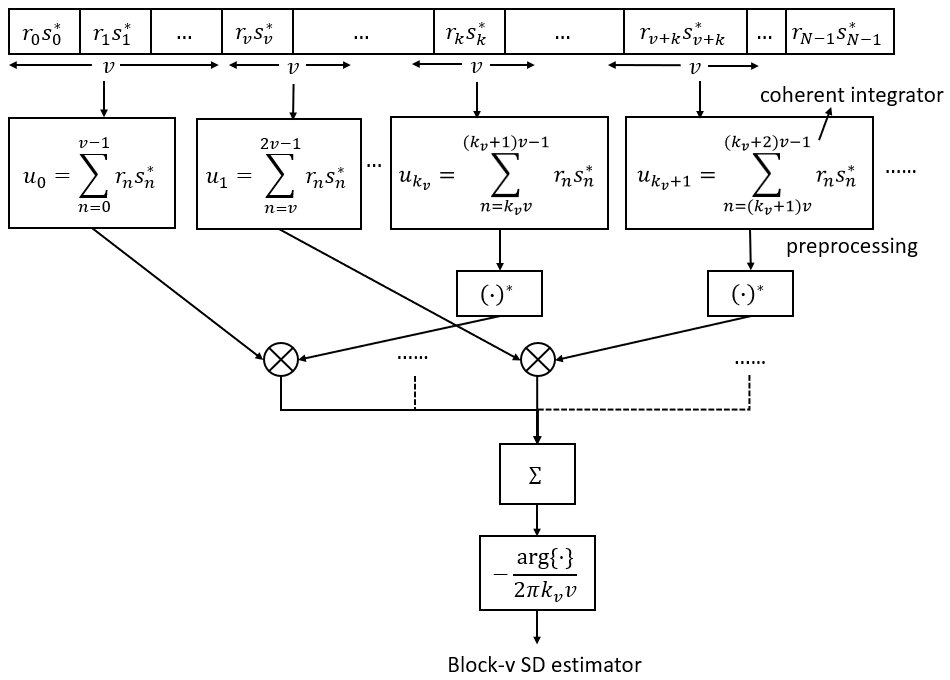
\includegraphics[width=3.4in,height=3.2in]{general_SD_estimator.png}}
  \caption{Flow diagram of implementing the Block-$v$ SD estimator}
  \label{fig:general_SD_estimator}
  \end{figure}

The reason for primary SD est-imator in~\eqref{eq:delta_SD} has a relatively bad performance at low SNR is due to the large noise
disturbance that greatly decorrelates the received signal and reference signal at every sample instant.
An alternative SD estimator is proposed by changing the order of computation in~\eqref{eq:delta_SD}.
Specifically, instead of calculating the correlation at each time instant and then averaging, we first do averaging of 
correlations for coherent time instants. The averaged results are called coherent integrators and the process is preprocessing; Then, use the remaining processing gain to integrate 
the coherent integrator between non-coherent time instants.
The details are illustrated in Figure~\ref{fig:general_SD_estimator}. 

In Figure~\ref{fig:general_SD_estimator}, the coherent integrator $u_l$ is formulated by

\begin{equation}
  \label{eq:coherent_integrator}
  u_l=\sum_{n=lv}^{(l+1)v-1}r_ns_n^*, \quad \text{for}~l=0,1,\ldots,N/v-1
\end{equation}
where $v$ is the block size of cross-correlation between received and reference signals. $v$ is set to be a factor of $N$
to include all sample instants.
$k_v$ denotes the distance between coherent integrator that calculates non-coherent cross-correlation.
Thus, $k_v=\lfloor k/v \rfloor$, where $\lfloor \cdot \rfloor$ represents the floor operation, since $v$ is not necessary to be a factor of $k$.
However, we still assume $k\approx k_vv$ for comparison simplicity. Based on above discussion, the alternative Block-$v$ SD estimator is given by

\begin{equation}
  \label{eq:general_sd_estimator}
  \hat{\delta}_{\text{Block}-v-\text{SD}}(v,k_v)=-\frac{\arg\big\{\sum_{l=k_v}^{N/v-1}u_l^*u_{l-k_v}\big\}}{2\pi k_vv}
\end{equation}
It can be seen that the primary SD estimator in~\eqref{eq:delta_SD} is a special case of Block-$v$ SD estimator when $v=1$.
Thus, we uniformly call the two estimators as Block-$v$ SD estimator.

Now, we discuss the performance of Block-$v$ SD estimator by focusing on the cross-correlation between the two coherent integrators in~\eqref{eq:general_sd_estimator}.
Based on~\eqref{eq:coherent_integrator} and the derivation of~\eqref{eq:ori_pdf_W}, the coherent integrator $u_l^*$ is complex Gaussian distributed with probability density function,

\begin{equation*}
  \label{eq:pdf_co_integrator_1}
  u_l^* \sim \cn\bigg(\frac{E_s/MS^*}{A^2}\sum_{n=lv}^{(l+1)v-1}e^{-j2\pi \bar{\delta}n},v\frac{E_s/M}{A^2}\frac{N_0}{2}\bigg),
\end{equation*}
and the pdf of complex Gaussian-distributed $u_{l-k_v}$ is also given by

\begin{equation*}
  \label{eq:pdf_co_integrator_2}
  u_{l-k_v} \sim \cn\bigg(\frac{E_s/MS}{A^2}\sum_{n=(l-k_v)v}^{(l-k_v+1)v-1}e^{j2\pi \bar{\delta}n},v\frac{E_s/M}{A^2}\frac{N_0}{2}\bigg).
\end{equation*}
Note, $u_l^*$ and $u_{l-k}$ are uncorrelated. Compared with~\eqref{eq:delta_extens_w_noise}, the cross-correlation between two coherent integrates $u_l^*$ and $u_{l-k_v}$ also yields a random variable
with a combination of Gaussian and second kind Bessel. The mean and variance of $u_l^*u_{l-k_v}$, denoted as $\mu_{C_u}$ and $\sigma^2_{C_u}$, are given by, respectively,

\begin{equation}
  \begin{aligned}
  \label{eq:cross_corr_co_inte}
  &\mu_{C_u}=\frac{(E_s/M)^2}{A^2}\sum_{n=lv}^{(l+1)v-1}e^{-j2\pi \bar{\delta}n}\sum_{m=(l-k)v}^{(l-k+1)v-1}e^{j2\pi \bar{\delta}m}, \\
  &\sigma^2_{C_u}=v^2\frac{(E_s/M)^2}{A^4}\Big(\frac{N_0}{2}\Big)^2+2v\frac{(E_s/M)^3}{A^4}\frac{N_0}{2}\Bigg(\frac{\sin(\pi \bar{\delta}v)}{\sin(\pi \bar{\delta})}\Bigg)^2,
\end{aligned}
\end{equation}
where $\frac{\sin(\pi \bar{\delta}v)}{\sin(\pi \bar{\delta})}$ is one of Dirichlet function, which approaches the maximum value $v$ at $\bar{\delta}=0$ and first pair of zero crossings at
$\bar{\delta}=\pm 1/v$. Based on~\eqref{eq:SNR_out_primary} and~\eqref{eq:cross_corr_co_inte}, 
the output SNR of Block-$v$ SD estimator in terms of the input SNR yields

\begin{equation}
  \begin{aligned}
    \label{eq:SNR_out_general}
    &\text{SNR}_{\text{out\_Blv}}=\frac{|\mu_{C_u}|^2}{\sigma^2_{C_u}} \\
    &=\frac{\frac{(Es/M)^4}{A^4}\Big(\frac{\sin(\pi \bar{\delta}v)}{\sin(\pi \bar{\delta})}\Big)^4(N/v-k_v)^2}
    {\Big[v^2\frac{(E_s/M)^2}{A^4}\Big(\frac{N_0}{2}\Big)^2+2v\frac{(E_s/M)^3}{A^4}\frac{N_0}{2}\Big(\frac{\sin(\pi \bar{\delta}v)}{\sin(\pi \bar{\delta})}\Big)^2\Big](N/v-k_v)} \\
    &=\frac{(N/v-k_v)\Big(\frac{\sin(\pi \bar{\delta}v)}{\sin(\pi \bar{\delta})}\Big)^4}
    {\frac{v^2}{\text{SNR}_{\text{in}}^2}+\frac{2v}{\text{SNR}_{\text{in}}}\Big(\frac{\sin(\pi \bar{\delta}v)}{\sin(\pi \bar{\delta})}\Big)^2}.
  \end{aligned}
\end{equation}
Some important observations of $\text{SNR}_{\text{out\_Blv}}$ from~\eqref{eq:SNR_out_general} can be discussed. 
First, $\text{SNR}_{\text{out\_Blv}}$ depends on the value of $|\bar{\delta}|v$.
We start to consider the case when $|\bar{\delta}|v\ll1$, i.e., $\frac{\sin(\pi \bar{\delta}v)}{\sin(\pi \bar{\delta})} \approx v$
and $(N/v-k_v)v \approx N-k$.
When the input SNR is moderate, the second term of variance dominates and results the same output SNR as in~\eqref{eq:SNR_out_primary};
While at low SNR, the first term of variance dominates and produces a $v$ times larger output SNR than primary SD estimator, which corresponds to the design intention of block-$v$ ($v \geq 2$) SD estimator.
Thus, the selection of $v$ trades off the processing gain at low SNR and the incurred large frequency offset.

By comparing~\eqref{eq:SNR_out_primary} and~\eqref{eq:SNR_out_general}, it can be seen that Block-$v$ SD estimator produces a positive processing gain both at low and high SNR, when $|\bar{\delta}|v$ satisfies
$v^{3/4}\leq\frac{\sin(\pi \bar{\delta}v)}{\sin(\pi \bar{\delta})}\leq v$; While, Block-$v$ SD estimator
only produces positive processing gain at high SNR with $\sqrt{v}\leq\frac{\sin(\pi \bar{\delta}v)}{\sin(\pi \bar{\delta})}<v^{3/4}$.
However, the worst case happens when $|\bar{\delta}|v_{\text{min}}$ even also produces a relative large frequency offset, 
i.e., $v_{\text{min}}=2$ and $0\leq\frac{\sin(2\pi \bar{\delta})}{\sin(\pi \bar{\delta})}<\sqrt{2}$. Then, the Block-$v$ SD estimator will suffer a worse performance than the primary SD estimator for all SNRs.

Now, let's measure the distribution of Block-$v$ SD estimator at low SNR.
Assume $|\bar{\delta}|v$ always satisfies $v^{3/4}\leq\frac{\sin(\pi \bar{\delta}v)}{\sin(\pi \bar{\delta})}\leq v$,
and the extra processing gain $v$ at relatively low SNR increases the $\text{SNR}_{\text{out\_Blv}}$ to meet the moderate SNR requirement of~\eqref{eq:sol_pdf_W}.
Thus, by plugging~\eqref{eq:cross_corr_co_inte},~\eqref{eq:sol_pdf_W} into~\eqref{eq:general_sd_estimator}, the block-$v$ SD estimator is distributed approximately Gaussian at relatively low SNR with probability density function

\begin{equation}
  \begin{aligned}
  \label{eq:pdf_general_delta}
      \est{\delta}{\text{Block}-v-\text{SD}}(&v,k_v) \\
      &\sim \n \bigg(\bar{\delta},\frac{M^2v^2}{16\pi^2k^2\Big(\frac{\sin(\pi \bar{\delta}v)}{\sin(\pi \bar{\delta})}\Big)^4(N/v{-}k_v)(E_s/N_0)^2}\bigg).
  \end{aligned}
\end{equation} 
Thus, $\est{\delta}{\text{Block}-v-\text{SD}}$ is also unbiased. Moreover, the lag $k_v$ also affects the variance of Block-$v$ SD estimator. The best choice is to choose
$k_v=\lfloor\frac{2N}{3v}\rfloor$ to minimize the variance. However,
it should be noted that if $k_v$ is too large, the frequency estimate $\est{\delta}{\text{Block}-v-\text{SD}}$ 
may be one of the alias of $\bar{\delta}$ if $2\pi|\bar{\delta}|k_vv>\pi$. The ambiguity problem is 
common in frequency estimation and we propose a method based on Chinese reminder theorem that solves this problem in the next section.
It shows that by some extra simple computation, $k_v$ can be chosen always by the optimal value. 

\subsubsection{Solution to preventing "alaising" of choice $k_v$}

The relat-ionship between frequency estimate $\hat{\delta}$ and true frequency offset $\bar{\delta}$ is given by 

\begin{equation}
  \label{eq:relationship_est_and_true_delta}
  2\pi \hat{\delta}k_vv+2\pi n=2\pi \bar{\delta}k_vv, \quad \text{for}~n=0,\pm 1,\pm 2,\ldots
\end{equation}
where $\hat{\delta}$ should satisfy $-\pi \leq 2\pi \hat{\delta}k_vv \leq \pi$. Thus, the ambiguity happens when $2\pi|\hat{\delta}k_vv|<\pi$ and~\eqref{eq:relationship_est_and_true_delta} doesn't holds for $n=0$.
To solve the ambiguity problem based on knowing the value of frequency estimate $\hat{\delta}$, we can obtain the true frequency offset $\bar{\delta}$ by 



% \subsubsection{Low-SNR Improvement}
% Recall that the expression of SD estimator with optimal choice $k$ only fits a moderate SNR.
% The performance of SD at low SNR is also crucial and needs to be discussed.
% One way to improving the accuracy is by averaging $K$ estimates of SD with different lags $k$.
% We call the resulting estimator the $K-$SD estimator, $\est{\delta}{K\text{-SD}}$.
% In this case, we trade off a $K$-fold increase in computational complexity for lower variance.

% Let $\bm{u}$ be a vector of non-negative, with
% $\sum_{k \in {\cal K}}u_k=1$; here ${\cal K}$ represents the set of $K$
% lags to be averaged.
% % extension to reviewer 1, comment 5, reviewer 3, comment 4
% Simple linear combining of $K$ SD estimators yields the $K-$SD estimator

% \begin{equation}
%   \label{eq:K_SD_est}
%       \est{\delta}{K\text{-SD}}=\sum_{k \in \cal K}\est{\delta}{\sd}(k)u_k.
% \end{equation}
% The optimal weight vector $\bm{u}_\opt$ can be obtained by minimizing the variance of $\est{\delta}{K\text{-SD}}$,
% which is well-known as

% \begin{equation}
%   \label{eq:u_opt}
%       \bm{u}_\opt=\frac{\bm{C}^{-1}\bm{1}}{\bm{1}^T\bm{C}^{-1}\bm{1}}.
% \end{equation}
% $\bm{C}$ is the autocovariance matrix between the $K$ SD estimators and $\bm{1}$ represents the column vector of one. 
% Unfortunately, it is generally difficult to know the full information of $\bm{C}$. However,
% If the lags $k \in {\cal K}$ are chosen to satisfy the spacing between any pair is at least
% equal to the oversampling factor $M$, then the estimates to be combined are approximately uncorrelated and unbiased; The  
% resulting $\bm{C}$ is a diagonal matrix of variance of each SD estimator. For example, a good choice for selecting 3 lags is 
% ${\cal K}=\{k_\opt-M,k_\opt,k_\opt+M\}$. The optimal weights $\bm{u}_\opt$ are proportional to the inverse of the
% variances in~\eqref{eq:pdf_delta}.

\subsection{Solution II: Newton-Method (NM) Estimator}

The SD estimator emphasizes low-complexity property and is intended to provide merely sufficiently good carrier synchronization
to enable coherent detection. Once the signal has been acquired, the SD estimator can be improved by 
investing additional computations. Since detection events are rare, the computational complexity is of little concern.

The principle is to use the SD (or $K-$SD) estimator as the starting point for a Newton-type iteration 
aimed at finding a better solution to the necessary condition~\eqref{eq:delta}. 
In principle, multiple iterations are possible to produce successively better approximations to the root of
$\J(\hat{\delta})$ in~\eqref{eq:delta}. Specifically, the iterations are given by

\begin{equation}
    \label{eq:iter_NM_est}
    \est{\delta}{\nm}^{(i+1)}=\est{\delta}{\nm}^{(i)}-
    \frac{\J(\est{\delta}{\nm}^{(i)})}{\J^\prime(\est{\delta}{\nm}^{(i)})}
  \end{equation}
where $\est{\delta}{\nm}^{(0)}~{=}~\est{\delta}{\sd}(k_{\opt})$ is the starting point of the iteration and
$\J^\prime(\cdot)$ denotes the derivative of $\J$ with respect to $\hat{\delta}$. Specifically,

\begin{equation}
    \label{eq:derivative of delta}
    J^\prime(\hat{\delta}) = \Im\bigg\{\sum_{k=1}^{N-1}{\sum_{m=k}^{N-1}{j2\pi k^2r_{m-k}r_m^{*}s_{m-k}^{*}s_m}e^{j2\pi\hat{\delta}k}}\bigg\}.
    \end{equation}
Our simulations indicate that only a single iteration is usually sufficient to achieve very good accuracy.


